\documentclass[aspectratio=169]{beamer}

\usetheme[progressbar=frametitle]{metropolis}
\usepackage{appendixnumberbeamer}
\usepackage{booktabs}
\usepackage[scale=2]{ccicons}
\usepackage{xspace}
\usepackage{caption}
\usepackage{subcaption}
\usepackage{amsmath, amssymb}

\title{Занятие 9: Градиентный спуск и искусственные нейроны}
\date{19 ноября 2022}

\begin{document}
\maketitle

\begin{frame}{Вспоминаем линейную регрессию}
    \begin{columns}
        \begin{column}{.3\linewidth}
            \[ y(x) = w_1 x + w_0 \]
        \end{column}
        \begin{column}{.69\linewidth}
            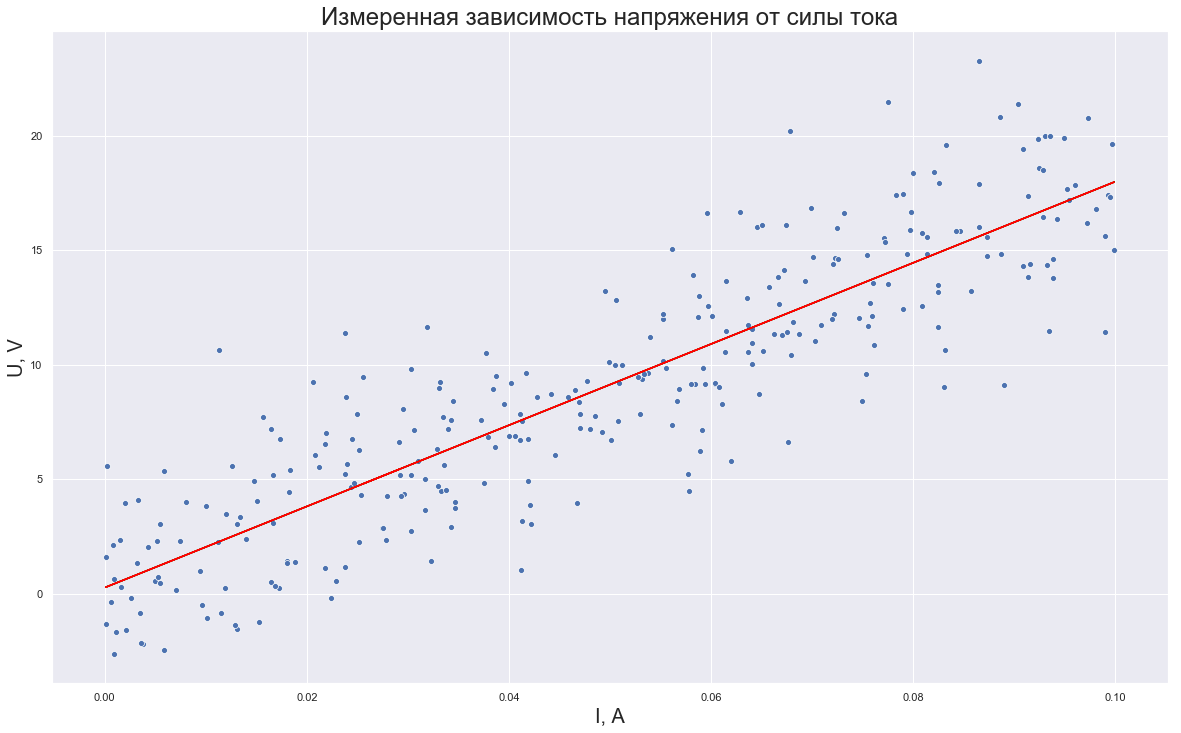
\includegraphics[width=\linewidth]{graphs/fig1.png}
        \end{column}
    \end{columns}
\end{frame}

\begin{frame}{Вспоминаем линейную регрессию}
    \centering{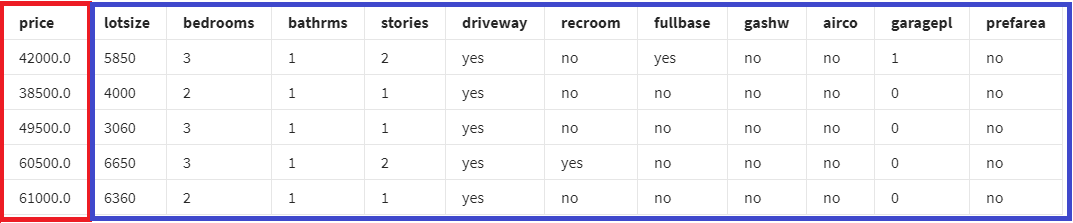
\includegraphics[width=.7\linewidth]{graphs/fig2.png}}
		\[ m = 11 \quad \textcolor{red}{\hat{y}(x)} = \sum_{i=0}^{m} w_i \textcolor{blue}{x_i} \]
		\[
			\textcolor{red}{\vec{y} = 
				\begin{pmatrix}
					y_1 \\ \vdots \\ y_N
				\end{pmatrix}}
			\quad
			\textcolor{blue}{X = 
				\begin{pmatrix} 
					1 & x_{11} & \cdots & x_{1m} \\ 
					\vdots & \vdots & \ddots & \vdots \\ 
					1 & x_{N1} & \cdots & x_{Nm} 
				\end{pmatrix}} 
			\quad
			\vec{w} = 
				\begin{pmatrix} 
					w_0 \\ 
					\vdots \\ 
					w_m 
				\end{pmatrix}
		\]
		\[ \textcolor{red}{\hat{\vec{y}}} = \textcolor{blue}{X} \vec{w} \]
\end{frame}

\begin{frame}{Вспоминаем линейную регрессию}
    \begin{columns}
        \begin{column}{.4\linewidth}
            Обучение:
            \[\mathcal{L}_{MSE}(y, \hat{y}) = \frac{1}{N} \sum_{i=1}^{N} {(y_i - \hat{y}_i)}^2\]
            \[ \vec{w}^* = \underset{w}{\arg\min} \mathcal{L} \]
            Аналитическое решение: \[ \vec{w}^* = {(X^T X)}^{-1} X^T y \]
        \end{column}
        \begin{column}{.5\linewidth}
            \centering
            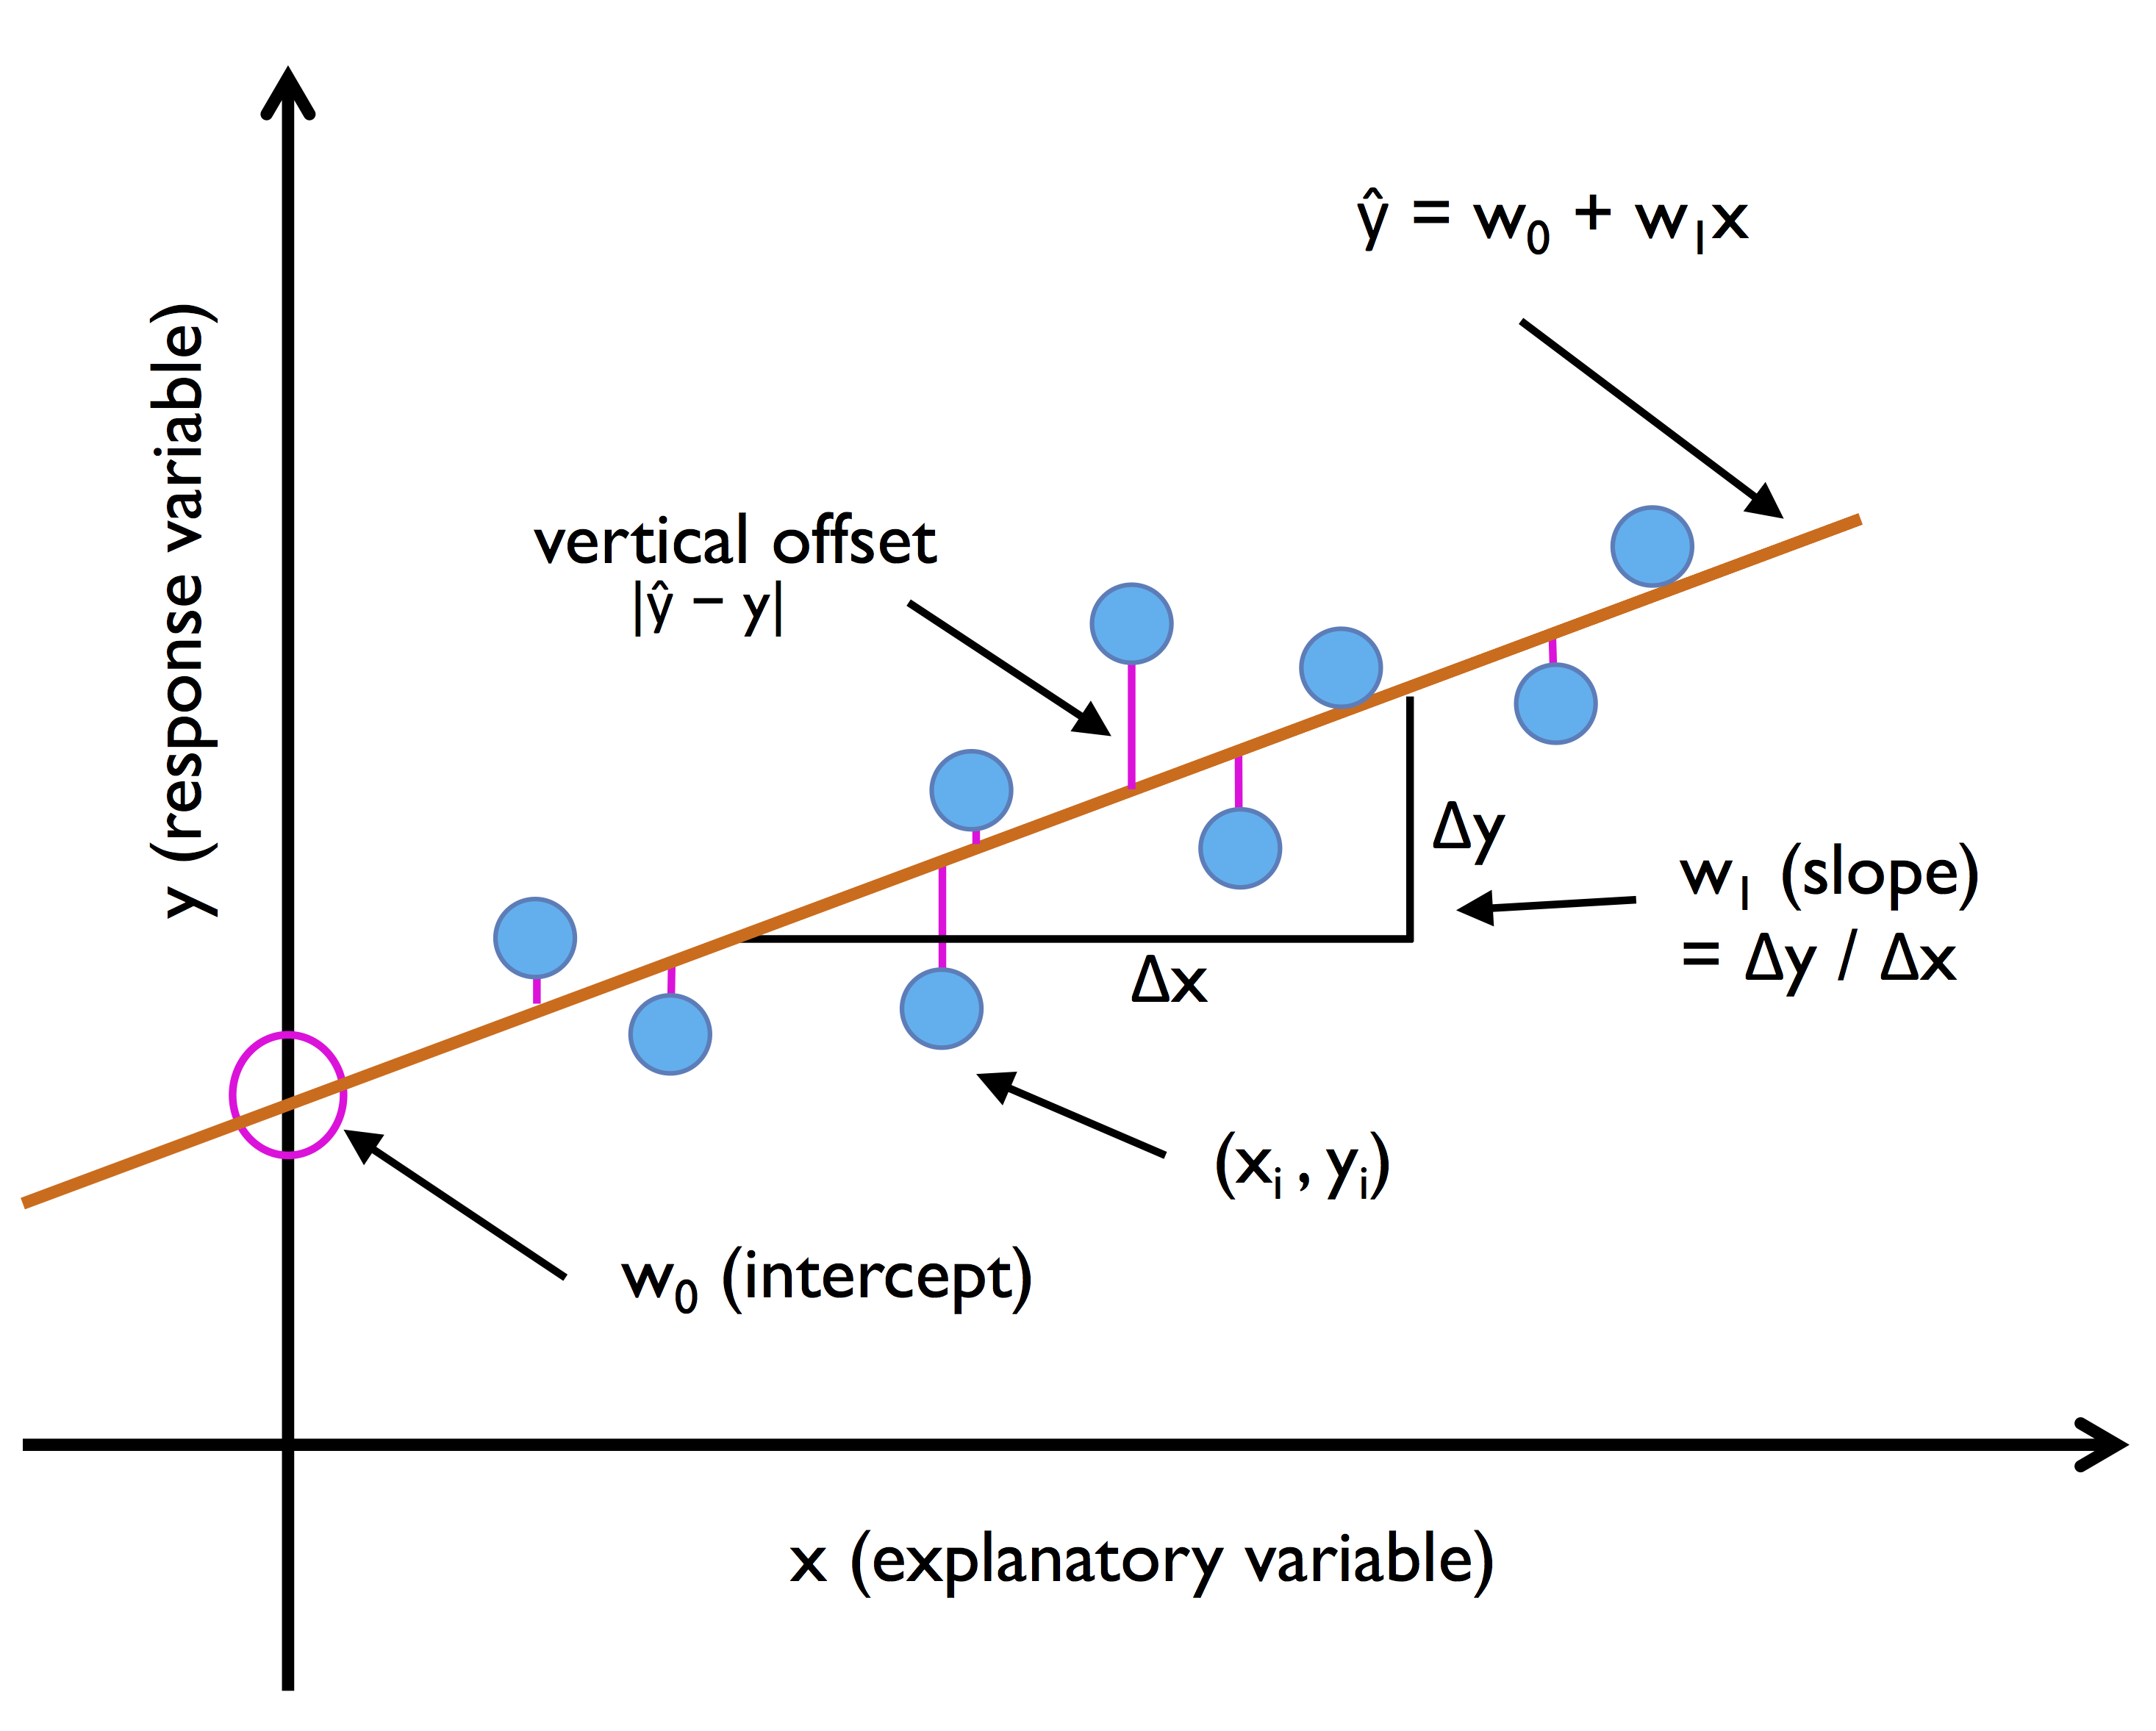
\includegraphics[width=\linewidth]{graphs/fig3.png}
        \end{column}
    \end{columns}
\end{frame}

\begin{frame}{Проблемы нахождения решения}
    \large{\[ \vec{w}^* = {(X^T X)}^{-1} X^T y \]}
    \begin{itemize}
        \item Может ли быть так, что формула выше неприменима?
        \pause
        \item Может ли быть так, что никакой формулы нет?
        \pause
        \item Что в таком случае делать?
        \pause
        \item Наивный вариант: перебор по сетке
        \item \(n = 100, m = 12 \rightarrow N_{ops} = 100^{12} = 10^{24}\)
    \end{itemize}
    \pause
    В таких случаях математика обращается к итеративным алгоритмам численной оптимизации.
\end{frame}

\begin{frame}{Градиентный спуск}
    \centering
	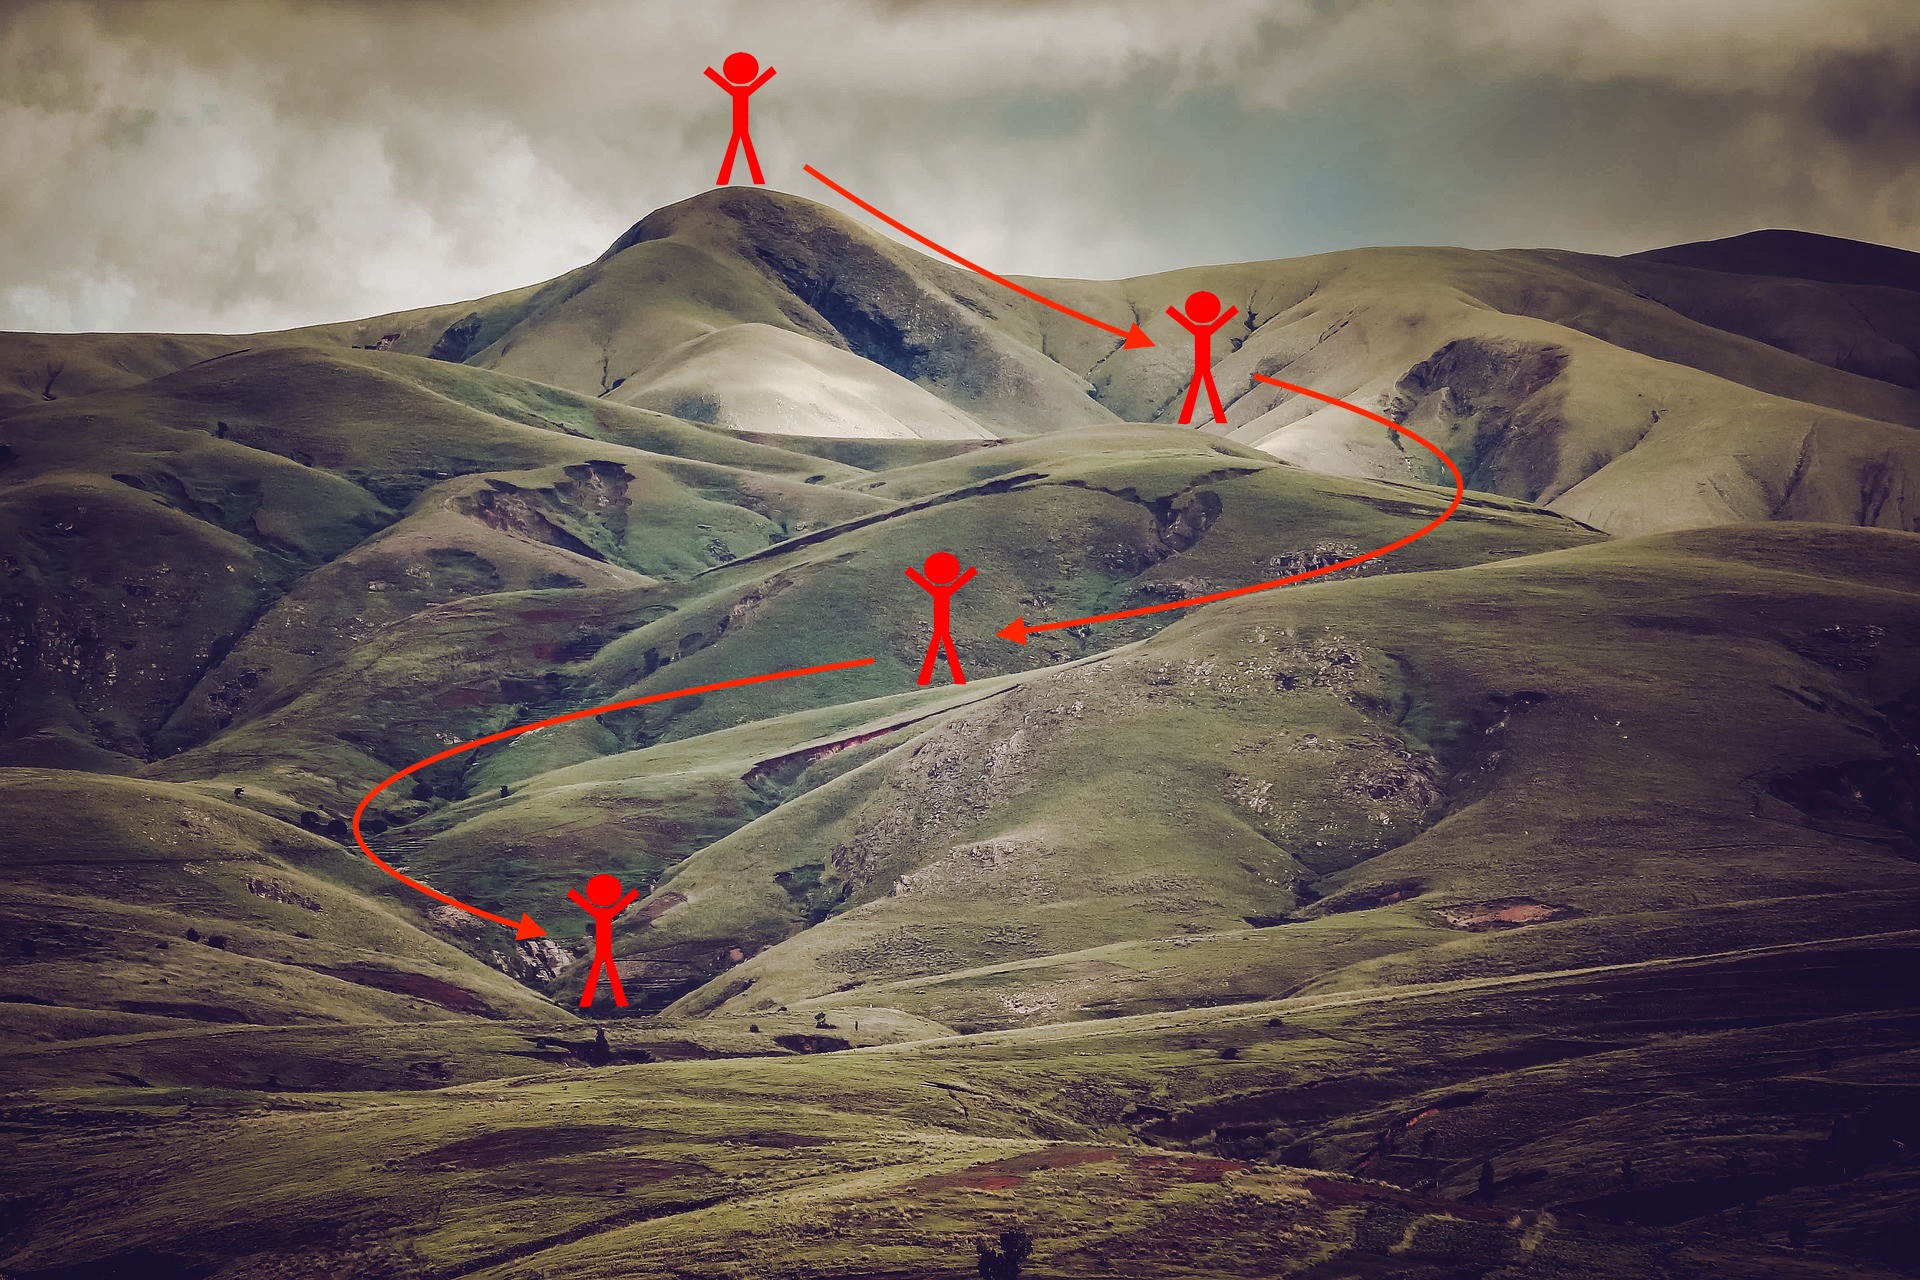
\includegraphics[width=.7\linewidth]{graphs/fig4.jpg}
\end{frame}

\begin{frame}{Градиентный спуск как метод оптимизации}
		\begin{columns}
			\begin{column}{.35\linewidth}
                Итеративный алгоритм:
                \[ w_{i, t+1} = w_{i, t} - \alpha \frac{\partial \mathcal{L}_t}{\partial w_i} \]
                В векторном виде:
                \[
                    \vec{\nabla} \mathcal{L}_t = \left(
                    \frac{\partial \mathcal{L}_t}{\partial w_1},
                    \frac{\partial \mathcal{L}_t}{\partial w_2},
                    \cdots
                    \right)
                \]
                \[ \vec{w}_{t+1} = \vec{w}_t - \alpha \vec{\nabla} \mathcal{L}_t \]
			\end{column}
			\begin{column}{.6\linewidth}
				\centering
				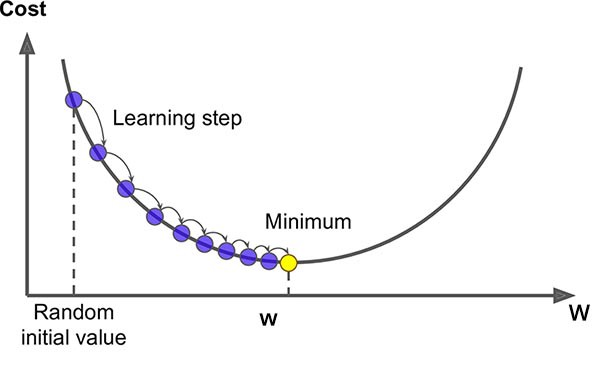
\includegraphics[width=\linewidth]{graphs/fig5.jpg}
			\end{column}
		\end{columns}
	\centering
	\(\alpha\) --- learning rate, шаг обучения (гиперпараметр)
\end{frame}

{
    \usebackgroundtemplate{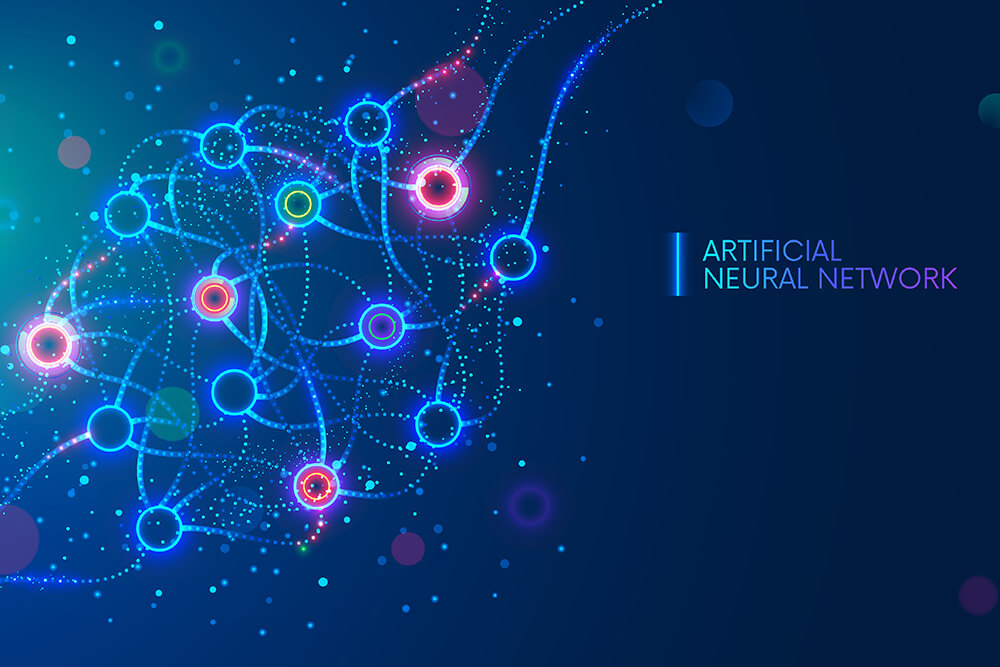
\includegraphics[width=\paperwidth]{graphs/fig6.jpg}}
    \begin{frame}
    \end{frame}
}

\begin{frame}{Биологические vs. искусственные нейроны}
    \begin{figure}
        \begin{subfigure}[b]{.4\linewidth}
            \centering
            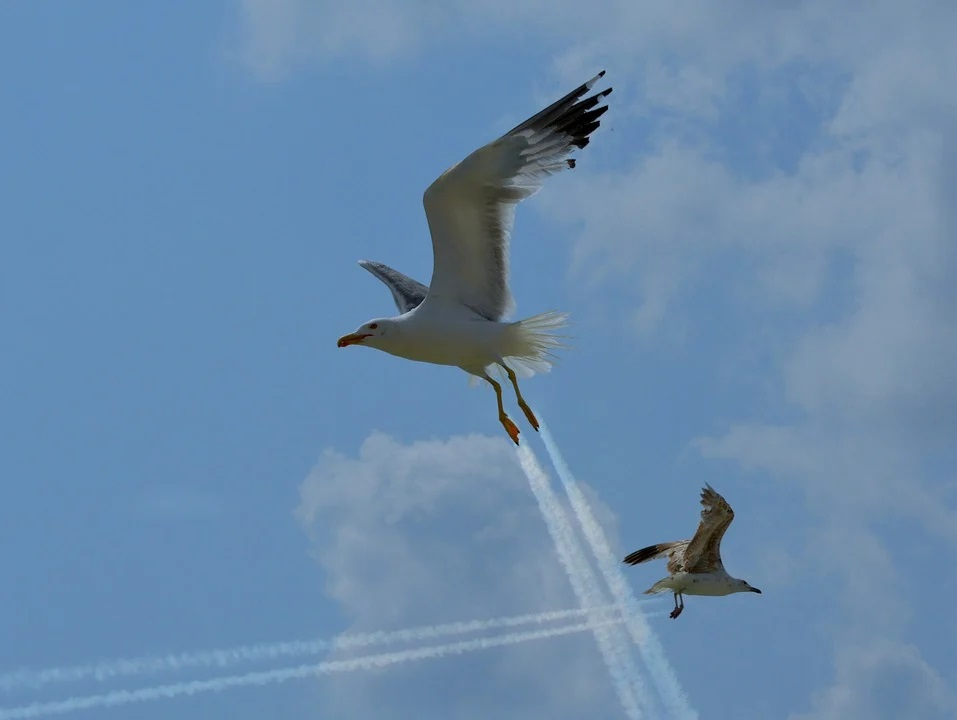
\includegraphics[width=\linewidth]{graphs/fig7.jpg}
            \caption*{Птица}
        \end{subfigure}
        \begin{subfigure}[b]{.59\linewidth}
            \centering
            
\includegraphics[width=.81\linewidth]{graphs/fig8.jpg}
            \caption*{Искусственная птица}
        \end{subfigure}
    \end{figure}
\end{frame}

\begin{frame}{Биологические vs. искусственные нейроны}
    \begin{figure}
        \begin{subfigure}[b]{.35\linewidth}
            \centering
            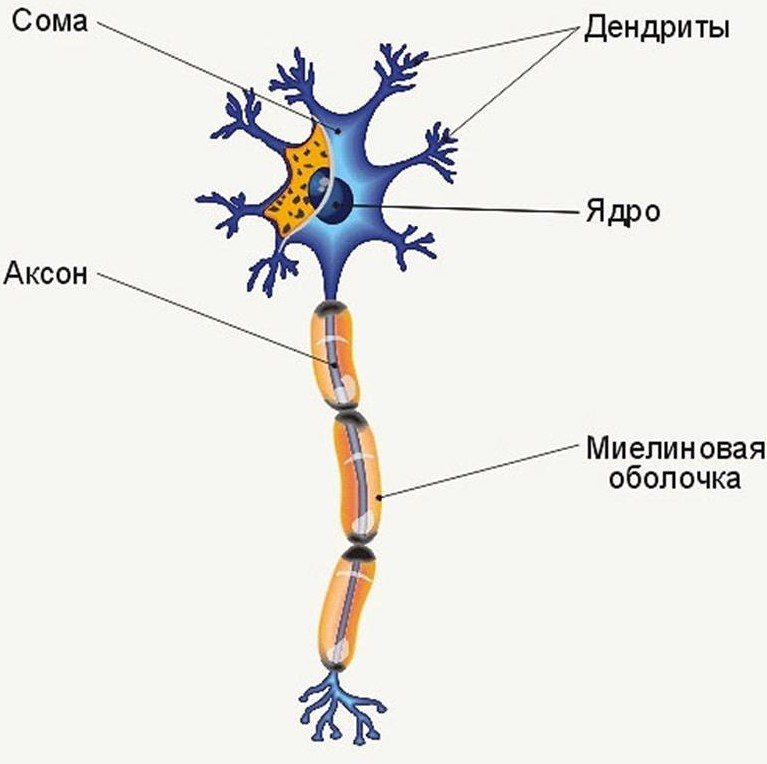
\includegraphics[width=\linewidth]{graphs/fig9.jpg}
            \caption*{Нейрон}
        \end{subfigure}
        \begin{subfigure}[b]{.64\linewidth}
            \centering
            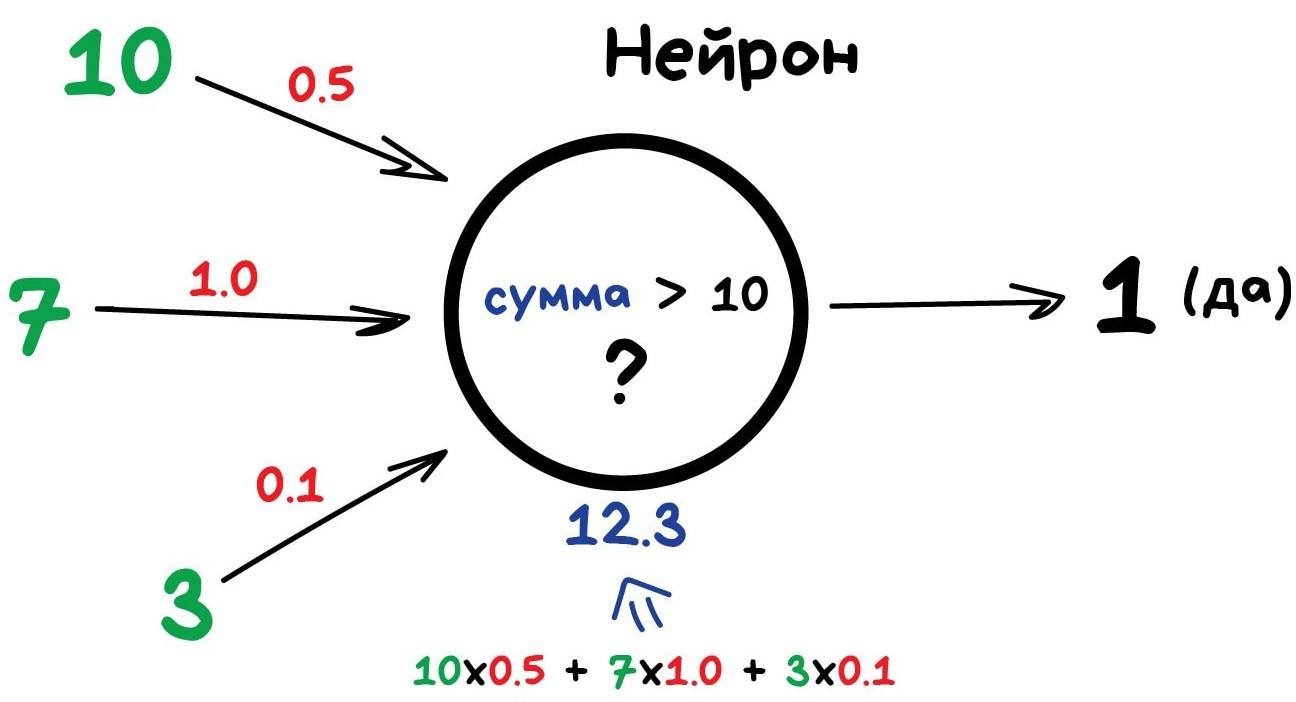
\includegraphics[width=\linewidth]{graphs/fig10.jpg}
            \caption*{Искусственный нейрон}
        \end{subfigure}
    \end{figure}
\end{frame}

\begin{frame}{Искусственный нейрон}
    \centering
    \small Матмодель нейрона: линейная регрессия + функция активации
    \[ n_{out} = f(w_0 + \sum^{m}_{i=1} w_i x_i) \]
    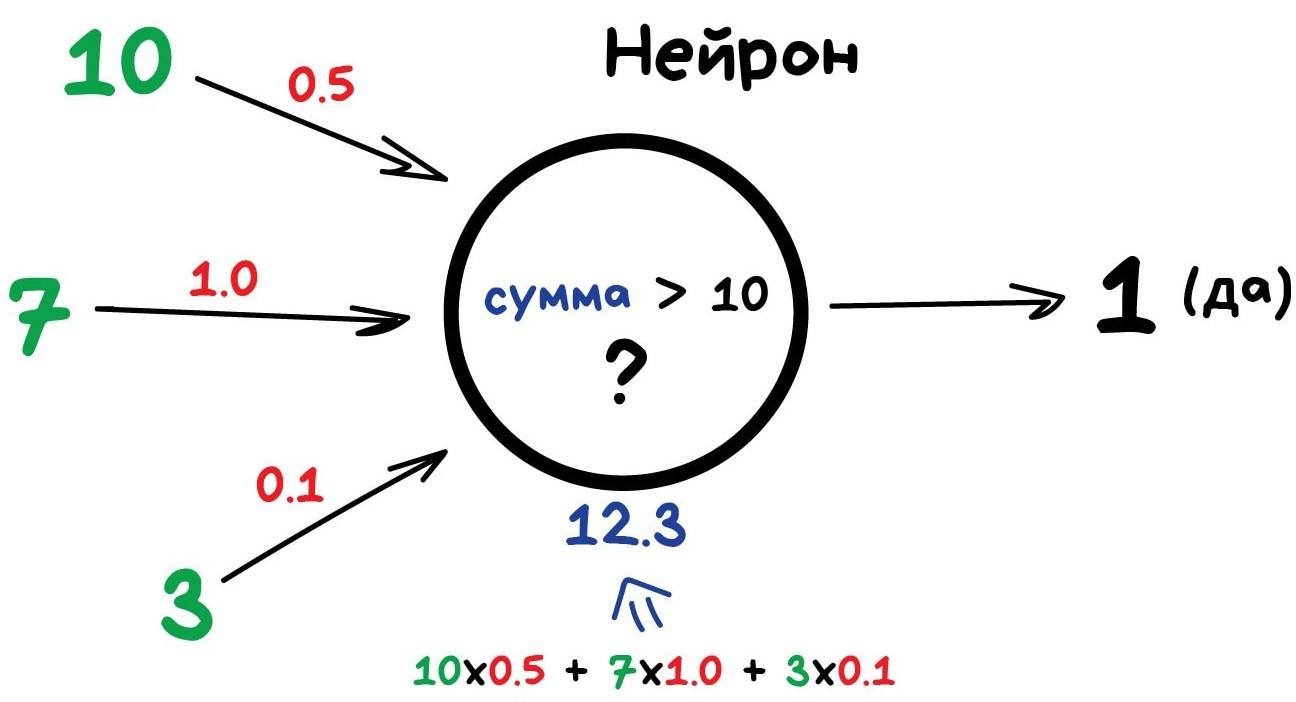
\includegraphics[width=.6\linewidth]{graphs/fig10.jpg}
\end{frame}

\begin{frame}{Функции активации}
    \small Функция активации --- нелинейная функция, применяемая к выходу сумматора
    \begin{figure}
        \begin{subfigure}[b]{.32\linewidth}
            \centering
            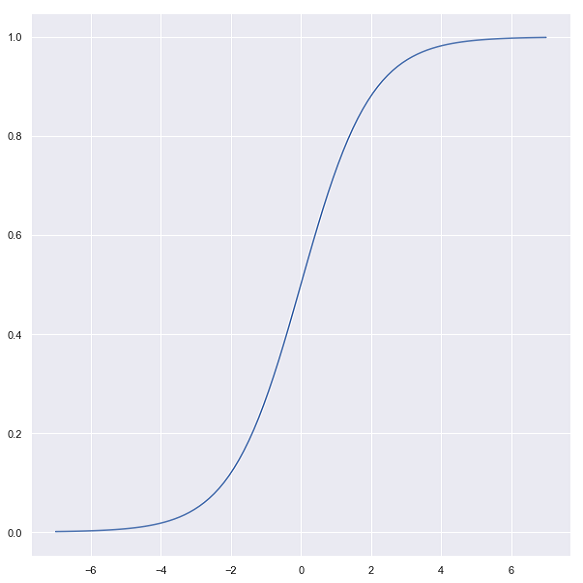
\includegraphics[width=\linewidth]{graphs/fig11.png}
            \subcaption*{\(\sigma (x) = \frac{1}{1 + e^{-x}}\)}
        \end{subfigure}
        \begin{subfigure}[b]{.32\linewidth}
            \centering
            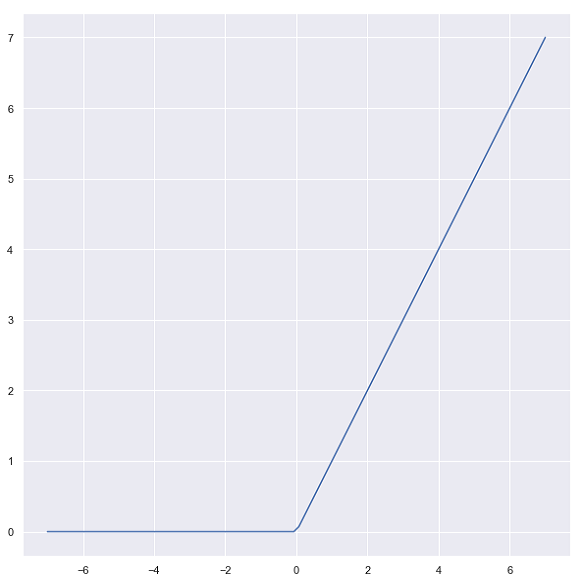
\includegraphics[width=\linewidth]{graphs/fig12.png}
            \subcaption*{\(ReLU(x) = \max(0, x)\)}
        \end{subfigure}
        \begin{subfigure}[b]{.32\linewidth}
            \centering
            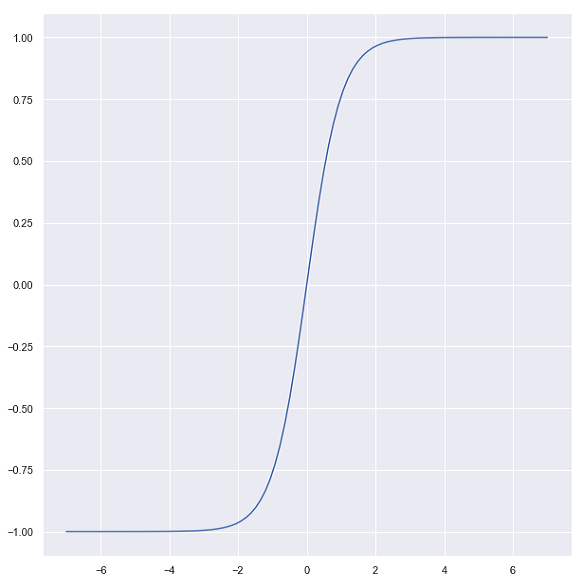
\includegraphics[width=\linewidth]{graphs/fig13.png}
            \subcaption*{\(\tanh(x)\)}
        \end{subfigure}
    \end{figure}
\end{frame}

\begin{frame}{Полносвязные нейронные сети}
    \centering
    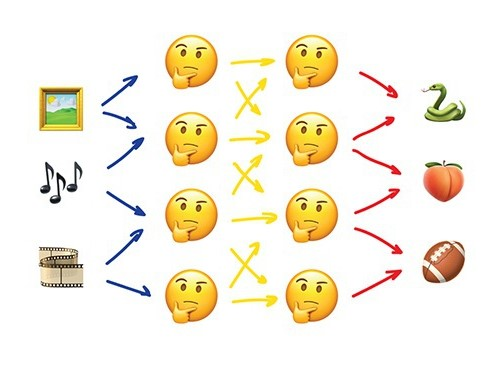
\includegraphics[width=.63\linewidth]{graphs/fig14.jpg}
\end{frame}

\begin{frame}{Нейронная сеть}
    \begin{columns}
        \begin{column}{.45\linewidth}
            \centering
            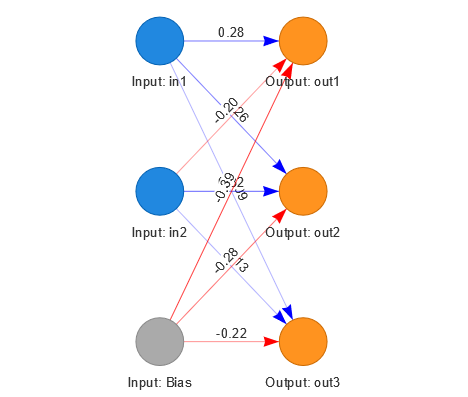
\includegraphics[width=\linewidth]{graphs/fig15.png}
            Однослойный перцептрон
        \end{column}
        \begin{column}{.5\linewidth}
            \centering
            \[
                \textcolor{red}{\vec{out} = 
                    \begin{pmatrix} 
                        out_1 \\ 
                        out_2 \\ 
                        out_3
                    \end{pmatrix}}
                \quad
                \textcolor{blue}{X =
                    \begin{pmatrix}
                        1 & in1_1 & in2_1 \\ 
                        \vdots & \vdots & \vdots \\ 
                        1 & in1_N & in2_N 
                    \end{pmatrix}} 
            \]
            \[
                W = 
                    \begin{pmatrix} 
                        b_1 & b_2 & b_3 \\ 
                        w_{11} & w_{12} & w_{13} \\ 
                        w_{21} & w_{22} & w_{23} 
                    \end{pmatrix} 
            \]
            \[ \textcolor{red}{\hat{\vec{out}}} = f(\textcolor{blue}{X} W) \]
            f применяется поэлементно
        \end{column}
    \end{columns}
\end{frame}

\begin{frame}{Полносвязная нейронная сеть}
    \begin{columns}
        \begin{column}{.45\linewidth}
            \centering
            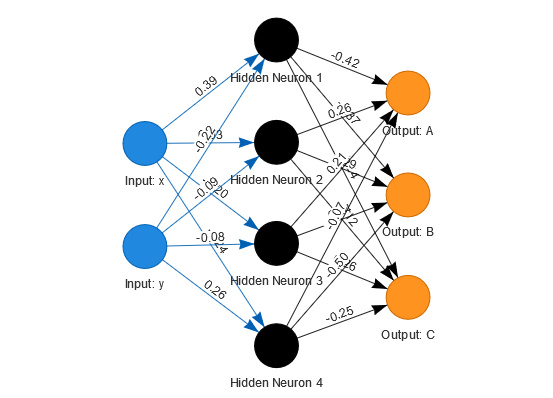
\includegraphics[width=\linewidth]{graphs/fig16.png}
            Сеть со скрытым слоем
        \end{column}
        \begin{column}{.5\linewidth}
            \small
            \centering
            \[
                \textcolor{red}{\vec{out} = \begin{pmatrix} A \\ B \\ C \end{pmatrix}}
                \quad
                \textcolor{blue}{X = 
                    \begin{pmatrix}
                        1 & x_1 & y_1  \\
                        \vdots & \vdots & \vdots \\
                        1 & x_N & y_N
                    \end{pmatrix}} 
            \]
            \[
                W_1 = 
                    \begin{pmatrix} 
                        b_1 & b_2 & b_3 & b_4 \\ 
                        w_{11} & w_{12} & w_{13} & w_{14} \\ 
                        w_{21} & w_{22} & w_{23} & w_{24}
                    \end{pmatrix}
                \quad
                H = f(\textcolor{blue}{X} W_1)
            \]
            \[
                W_2 = 
                    \begin{pmatrix} 
                        b_1 & b_2 & b_3 \\ 
                        w_{11} & w_{12} & w_{13} \\ 
                        w_{21} & w_{22} & w_{23}
                    \end{pmatrix} 
            \]
            \[ \textcolor{red}{\hat{\vec{out}}} = f(H W_2) = f(f(\textcolor{blue}{X} W_1) W_2) \]
        \end{column}
    \end{columns}
\end{frame}

\begin{frame}{Полносвязная нейронная сеть}
    \centering
    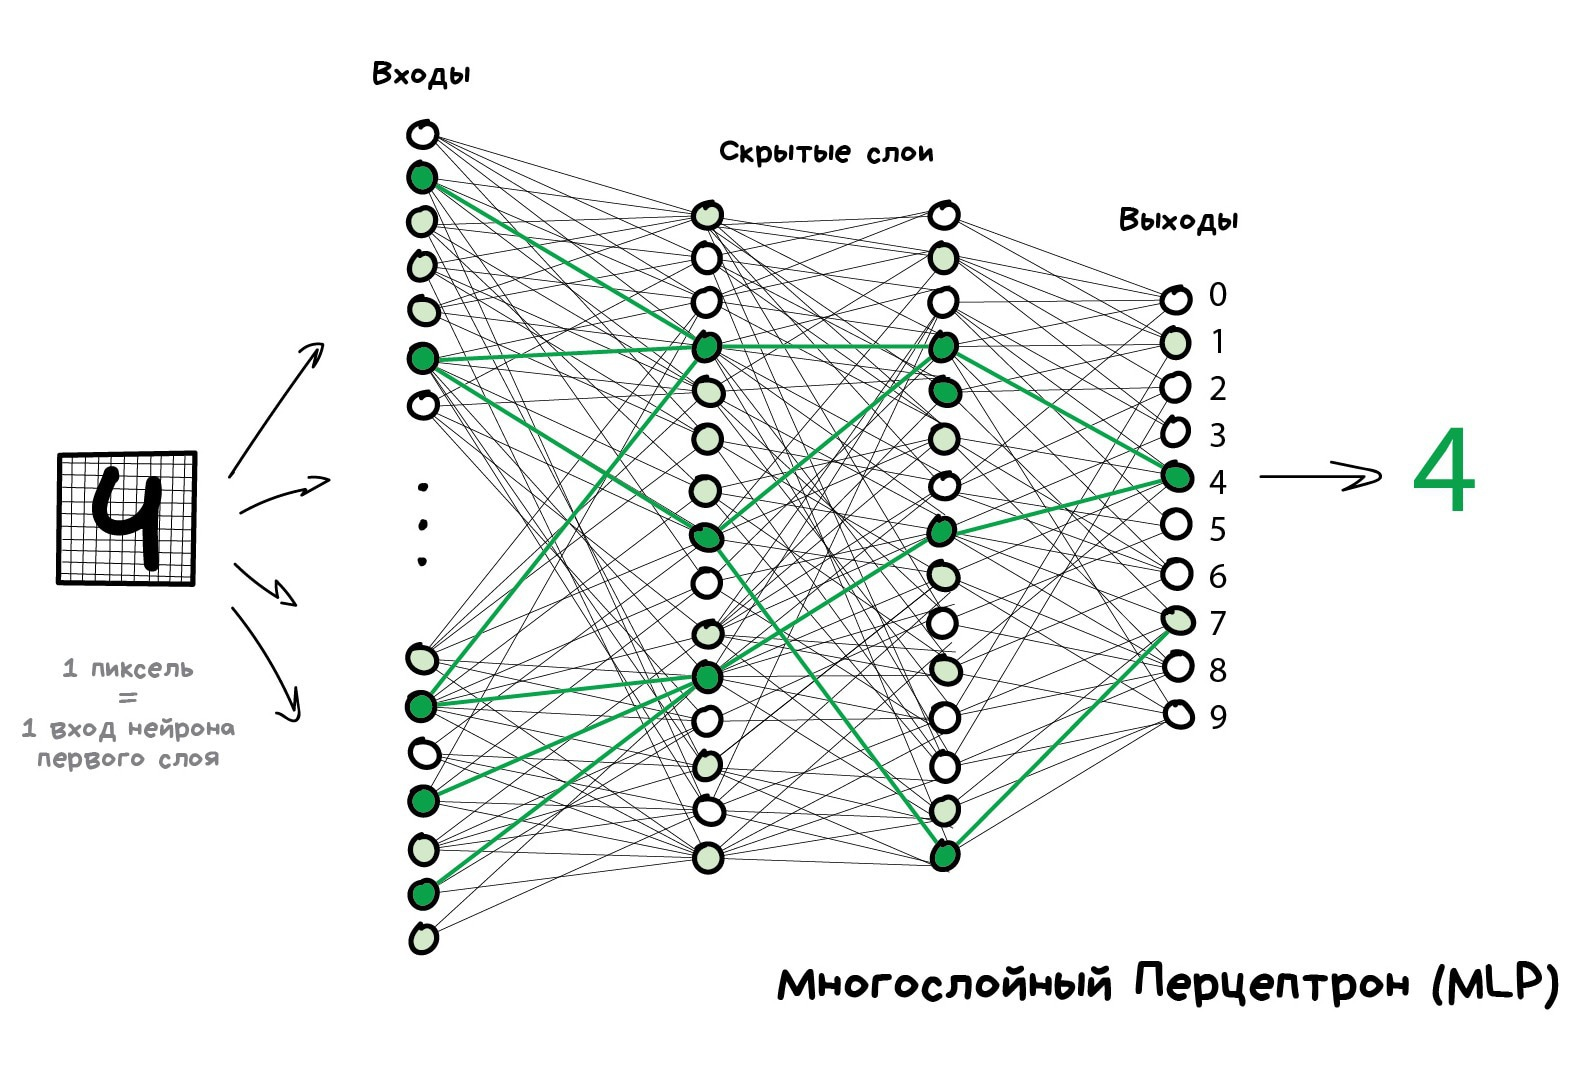
\includegraphics[width=.71\linewidth]{graphs/fig17.jpg}
\end{frame}

\end{document}